\documentclass{beamer}

\mode<presentation>

\usepackage[dutch]{babel}
%\usepackage{beamerthemesplit}
\usepackage{hyperref}

\usetheme{Berlin}
\useinnertheme{rounded}
\usecolortheme{rose}
\setbeamertemplate{navigation symbols}{} 
\title{Design patterns}
\author{W. Oele}
\date{\today}

\begin{document}
\frame{\titlepage}

\section{Design patterns}

\begin{frame}
\frametitle{Deze les}
\begin{itemize}
\item Het decorator patroon
\end{itemize}
\end{frame}


\begin{frame}
\frametitle{Het decorator pattern}
\begin{itemize}
\item naam: het decorator pattern
\item doel: extra verantwoorelijkheid toevoegen aan bestaande objecten en dit evt. dynamisch kunnen doen.
\item hoe: object ``inkapselen'' in abstracte parentklasse en decorators polymorphistisch afleiden.
\item gevolgen: extra verantwoordelijkheden kunnen dynamisch en in willekeurige volgorde worden toegevoegd.
\end{itemize}
\end{frame}

\begin{frame}
\frametitle{Het probleem: tegels maken}
De basis tegel\ldots wit
\begin{center}
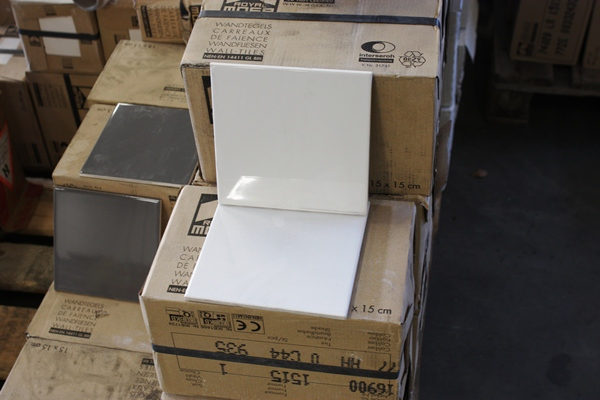
\includegraphics[width=6cm]{tegel1}
\end{center}
\end{frame}

\begin{frame}
\frametitle{Diverse varianten}
\begin{center}
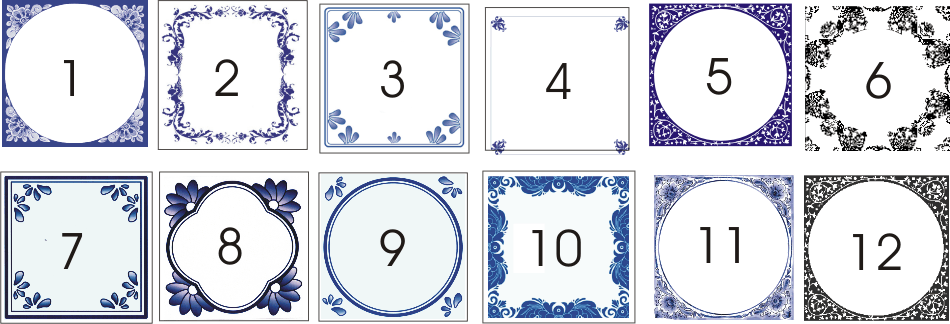
\includegraphics[width=8cm]{tegel2}
\begin{itemize}
\item met of zonder tekst
\item met of zonder rand
\item met of zonder versiersels in de hoeken
\item extra glazuur
\item etc.
\end{itemize}
\end{center}
\end{frame}

\begin{frame}
\frametitle{Het model}
\begin{center}
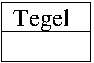
\includegraphics[width=2cm]{model1}
\end{center}
Verschillende ``decoraties'' kunnen door elkaar gebruikt worden:
\begin{itemize}
\item Een ketting van afgeleide klassen maken is dus geen goed idee.
\item Polymorphisme is eveneens geen goed idee.
\end{itemize}
\end{frame}

\begin{frame}
\frametitle{Het model}
\begin{center}
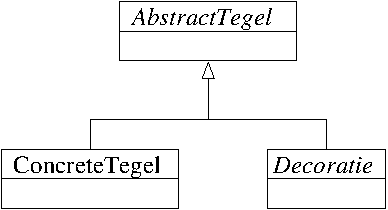
\includegraphics[width=6cm]{model2}
\end{center}
\end{frame}

\begin{frame}
\frametitle{Het model}
\begin{center}
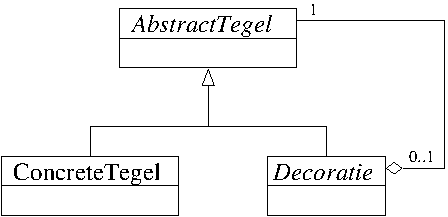
\includegraphics[width=6cm]{model3}
\end{center}
\end{frame}

\begin{frame}
\frametitle{Het model}
\begin{center}
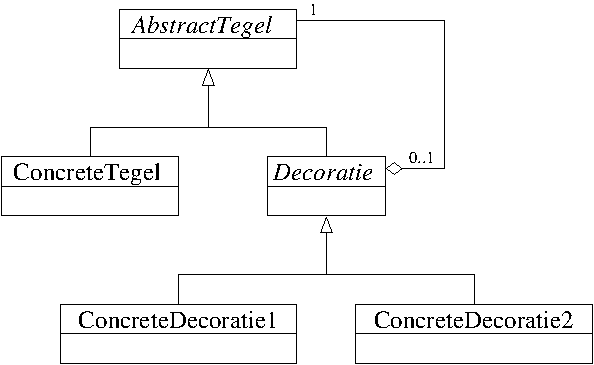
\includegraphics[width=8cm]{model4}
\end{center}
\end{frame}

\begin{frame}
\frametitle{Methodes}
\begin{center}
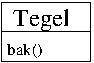
\includegraphics[width=2cm]{model5}
\end{center}
\end{frame}

\begin{frame}
\frametitle{Methodes}
\begin{center}
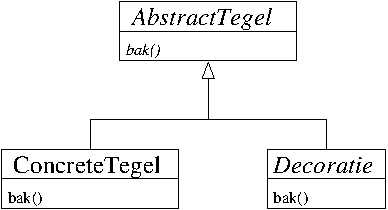
\includegraphics[width=6cm]{model6}
\end{center}
\end{frame}

\begin{frame}
\frametitle{Methodes}
\begin{center}
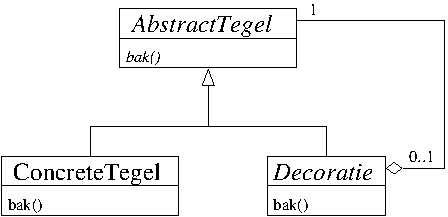
\includegraphics[width=8cm]{model7}
\end{center}
\end{frame}

\begin{frame}
\frametitle{Methodes}
\begin{center}
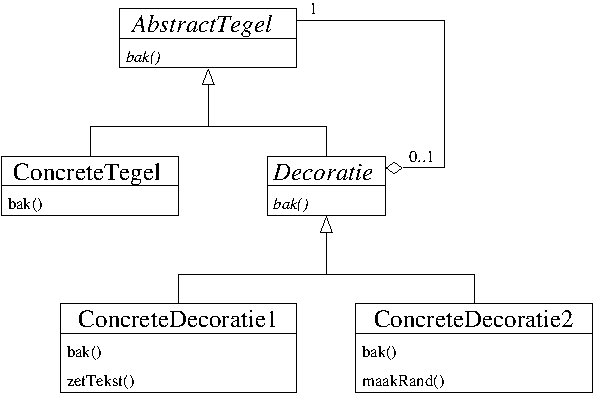
\includegraphics[width=8cm]{model8}
\end{center}
\end{frame}

\begin{frame}[fragile]
\frametitle{Code}
\begin{verbatim}
public abstract class AbstractTegel
{
   public abstract void bak();
}
\end{verbatim}
\end{frame}

\begin{frame}[fragile]
\frametitle{Code}
\begin{verbatim}
public class ConcreteTegel extends AbstractTegel
{
   @override
   public abstract void bak()
   {
      //standaard tegeltje bakken...
   }

}
\end{verbatim}
\end{frame}


\begin{frame}[fragile]
\frametitle{Code}
\begin{verbatim}
public abstract class Decoratie extends AbstractTegel
{
   private Tegel mijntegel;

   public Decoratie(AbstractTegel t)
   {
      mijntegel=t;    
   }
   
   public void bakTegel()
   {
      if(mijntegel!=null)mijntegel.bak();
   }
}
\end{verbatim}
\end{frame}



\begin{frame}[fragile]
\frametitle{Code}
\begin{verbatim}
public class ConcreteDecoratie1 extends Decoratie
{
   public ConcreteDecoratie2(AbstractTegel t)
   {
      super(t);
   }

   public void bak()
   {
      super.bakTegel();
      //extra code voor deze decoratie
   }   
}
\end{verbatim}
\end{frame}



\end{document}